\documentclass[paper=a4, fontsize=11pt]{scrartcl} % A4 paper and 11pt font size

%----------------------------------------------------------------------------------------
%	PACKAGES
%----------------------------------------------------------------------------------------
\usepackage[T1]{fontenc} % Use 8-bit encoding that has 256 glyphs
\usepackage{fourier} % Use the Adobe Utopia font for the document - comment this line to return to the LaTeX default
\usepackage[english]{babel} % English language/hyphenation
\usepackage{amsmath,amsfonts,amsthm} % Math packages
\usepackage{sectsty} % Allows customizing section commands
\usepackage{fancyhdr} % Custom headers and footers
\usepackage{tabularx, outlines, framed, varwidth, enumitem, graphicx, listings, color, qtree, float, subcaption, newfloat}
\usepackage[left=0.5in, right=0.5in, top=3in, bottom=.25in]{geometry}
\geometry{}

%----------------------------------------------------------------------------------------
%	SET CUSTOMIZATIONS AND FUNCTIONS
%----------------------------------------------------------------------------------------
\sectionfont{\centering \normalfont\scshape} % Make all sections centered, the default font and small caps
\pagestyle{fancyplain} % Makes all pages in the document conform to the custom headers and footers
\fancyhead{} % No page header - if you want one, create it in the same way as the footers below
\fancyfoot[L]{} % Empty left footer
\fancyfoot[C]{} % Empty center footer
\fancyfoot[R]{\thepage} % Page numbering for right footer
\renewcommand{\headrulewidth}{0pt} % Remove header underlines
\renewcommand{\footrulewidth}{0pt} % Remove footer underlines
\setlength{\headheight}{0pt} % Customize the height of the header

\DeclareFloatingEnvironment[fileext=lod]{diagram}

\numberwithin{equation}{section} % Number equations within sections (i.e. 1.1, 1.2, 2.1, 2.2 instead of 1, 2, 3, 4)
\numberwithin{figure}{section} % Number figures within sections (i.e. 1.1, 1.2, 2.1, 2.2 instead of 1, 2, 3, 4)
\numberwithin{table}{section} % Number tables within sections (i.e. 1.1, 1.2, 2.1, 2.2 instead of 1, 2, 3, 4)

\graphicspath{{./figures/}}
%\setlength\parindent{0pt} % Removes all indentation from paragraphs - comment this line for an assignment with lots of text

\makeatletter
	\newcommand*\variableheghtrulefill[1][.4\p@]
	{%
		\leavevmode
		\leaders \hrule \@height #1\relax \hfill
		\null
	}
\makeatother

\lstset
{
	language=C++,
%	basicstyle=\ttfamily,
%	keywordstyle=\color{blue}\ttfamily,
%	stringstyle=\color{red}\ttfamily,
%	commentstyle=\color{green}\ttfamily,
%	morecomment=[l][\color{magenta}]{\#}
	keywordstyle=\color{blue},
	stringstyle=\color{red},
	commentstyle=\color{green},
	morecomment=[l][\color{magenta}]{\#}
}

%----------------------------------------------------------------------------------------
%	USEFUL COMMANDS
%----------------------------------------------------------------------------------------
%	\makebox[\textwidth][c]{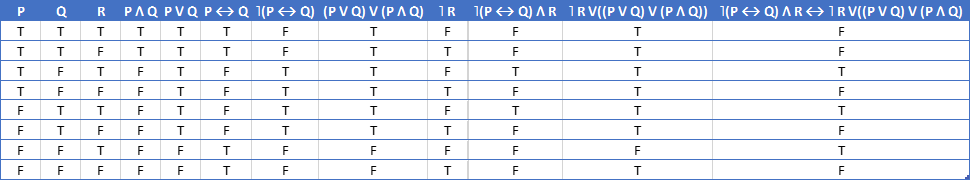
\includegraphics[width=.9\pagewidth]{p2-table}}

%	\newgeometry{top=.75in, bottom=.75in, left=.25in,right=.25in}
%	\newgeometry{top=.75in, bottom=.75in, left=1.25in,right=1.25in}

%	\lstinputlisting[firstline=4]{CMPSC360_Homework.cpp}

%\Tree
%	[.<root> [.<left> ][.<middle> ][.<right> ]]

%----------------------------------------------------------------------------------------
%	TITLE SECTION
%----------------------------------------------------------------------------------------

\newcommand{\horrule}[1]{\rule{\linewidth}{#1}} % Create horizontal rule command with 1 argument of height
% \title{Template: Homework 1}
\title{	
\normalfont \normalsize 
%\textsc{Rutgers University, Real Analysis I} \\ [25pt] % Your university, school and/or department name(s)
\horrule{0.5pt} \\[0.4cm] % Thin top horizontal rule
\huge CMPSC 448: Homework 4 \\ % The assignment title
\horrule{2pt} \\[0.5cm] % Thick bottom horizontal rule
}

\author{\textbf{\underline{Name:}}Kyle Salitrik | \textit{\textbf{\underline{ID\#:}} 997543474} | \textit{\textbf{\underline{PSU ID:}} kps168}} % Your name

\date{\normalsize\today} % Today's date or a custom date

\begin{document}

\maketitle % Print the title

%----------------------------------------------------------------------------------------
%	PROBLEM 1
%----------------------------------------------------------------------------------------
\newgeometry{top=.75in, bottom=.75in, left=1.25in,right=1.25in}
\section*{\variableheghtrulefill[.25ex]\quad Problem 2 \quad\variableheghtrulefill[.25ex]}

\subsection*{1) Centering}
\subsubsection*{What it means}
Centering is when you subtract the mean of each feature of the data from each individual data point.
\subsubsection*{Why it's important}
Centering is important because it allows the matrix decomposition in PCA to find the actua covariance matrix of the data and therefore find the eigenvectors with the highest variance.
 
\subsubsection*{How to apply it}
To apply centering:
\begin{align*}
	\boldsymbol{\mu} &= \frac{1}{n} \sum_{i = 1}^{n} \boldsymbol{x_i} &\\
	\boldsymbol{x_i} &= \boldsymbol{x_i} - \boldsymbol{\mu}&\\
\end{align*}

\subsection*{2) Scaling}
\subsubsection*{What it means}
Scaling is the transformation of data to a desired interval. It typically refers to normalization or standardization (discussed below).

\subsubsection*{Why it's important}
Scaling is important for PCA because simply having a feature vector with a larger scale than the other features will cause the PCA algorithm to identify that eigenvector to have the highest variance, although that may not be true.

\subsubsection*{How to apply it}
Scaling is typically done by applying a scalar multiplication to each feature vector, which can be shown as a Hadamard product:
\begin{align*}
	\boldsymbol{v'} = \boldsymbol{v^{\mathbb{R}^d}} \odot [s_1, s_2, s_3, ... , s_d]&&
\end{align*}

After these features are scaled they can then be shifted by adding a unique scalar value to each feature dimension. Any other linear operation or function can also be applied in a similar fashion.

\subsection*{3) Normalization}
\subsubsection*{What it means}
Normalization is when each feature dimension is scaled to be within the interval [0, 1]

\subsubsection*{Why it's important}
Normalization is important for a similar reason as discussed in the scaling section. If all of the features are normalized, then the PCA algorithm will treat them all as 'equal' when attempting to find the direction of highest variance. Using normalization avoids the algorithm assuming one feature is better than another simply because it's values are on a large scale.

\subsubsection*{How to apply it}
Normalization can be applied by shifting all of the data for each feature such that the minimum value is 0 and then dividing by the maximum value of that feature.

\subsection*{4) Standardization}
\subsubsection*{What it means}
Standardization is when each feature dimension is shifted to have a mean of zero and scaled to have a maximum range of one standard deviation in each direction.

\subsubsection*{Why it's important}
Standardization attempts to convert each feature dimension into a normal distribution. This is useful because the normal distribution is well understood and documented, as well as provides us a way to calculate things like the variance more easily.

\subsubsection*{How to apply it}
To apply standardization, the mean ($\mu_d$) and standard deviation ($\sigma_d$) of each feature dimension is calculated, and then the following equation is applied to all data points: 
\begin{align*}
	x'_{n,d} = \frac{x_{n,d} - \mu_d}{\sigma_d} &&
\end{align*}


\end{document}